\section{Feedback impl.}

\frame{

After several experiments came to this scheme with the summing amplifier:
\begin{center}
    \incfig{scheme3}
\end{center}

Photodiode power is enough to not use an additional amplifier. \frametitle{Scheme}}

% вставить слайд с вахами и картинками:
% хватает усилиения, 

% \frame{
% 
Makes sense to be in the most sensitive range, it was measured: \\
 -\ $I$-$V$ curve  for a laser \\
 -\ the dependence of the ph. diode voltage on the laser power.

\begin{figure}[h]
    % \centering
    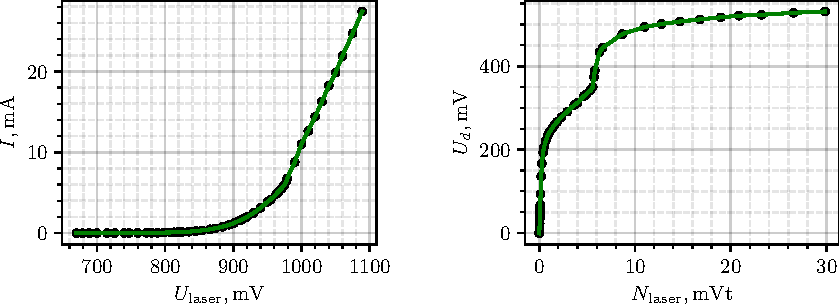
\includegraphics[width=1.0\textwidth]{figures/IV.pdf}
    %\caption{}
    %\label{fig:}
\end{figure}

So, laser voltage range of  $0.85$V selected. \frametitle{I–V curve}}

\frame{

Makes sense to be in the most sensitive range, it was measured: \\
 -\ $I$-$V$ curve  for a laser \\
 -\ the dependence of the ph. diode voltage on the laser power.

\begin{figure}[h]
    % \centering
    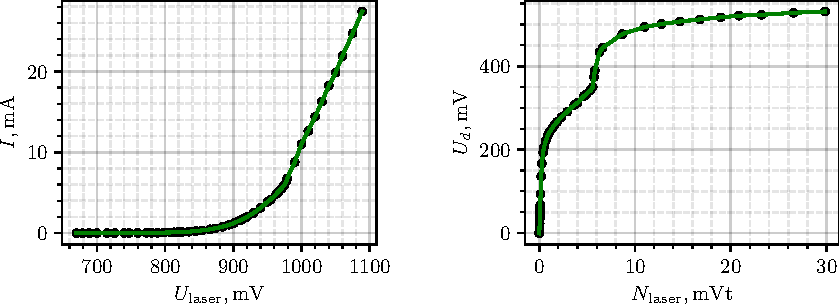
\includegraphics[width=1.0\textwidth]{figures/IV.pdf}
    %\caption{}
    %\label{fig:}
\end{figure}

So, laser voltage range of  $0.85$V selected. \frametitle{I–V curve}}

\frame{
For testing, the assembly was carried out on the dumping board.
\begin{center}
    \incfig{scheme4}
\end{center}

\hspace{-3mm}
\textbf{Thus, a scheme with positive feedback was implemented.} \\

\hspace{-3mm}
However, no desired oscillations were observed. \frametitle{Realization}}

% варьируя длина оптоволокна -- можем контролировать
% то что нашли -- маломощное, подходя к нужным мощностям всё же сжигали.
% научились стабилизировать оу, поняли необходимость аккура
% 
\frame{
With used amplifiers, the following oscillations at the amplifier output with DC power can be observed:

\begin{center}
    \incfig{scheme5}
\end{center}

This is due to the instability of the amplifier. 
% This instability can be eliminated by the adjustment of the scheme. 

\phantom{42}

The main problem is that desired oscillations $\sim 10$ ns. \\

\phantom{42}

We proceeded to experiments with faster amplifiers, but it is usefull to understand results of such delays.

oscillations megahertz
 \frametitle{Problems}}

% \frame{
% However, it was not possible to move to the chaotic regime in the laser. Possible cause of the problem may be
\begin{itemize}
    \iitem{parasitic capacity and inductance,}
\end{itemize}
In terms of solutions -- neatly soldered scheme.


% \phantom{42}

% A suitable amplifier, with similar properties used in the article, must come in June. \frametitle{Problems}}



% \frame{
% % слайд про то что: 
% или аккуратная схемотехника, или медленный лазер
%  \frametitle{Real system}}


